\section{Every system treats a completing deed as a rival's claim}
\label{sec:attention}

\subsection{Responses to offers}

The \fact{barg.census.threads} threads contain \fact{barg.census.responses-all.n} responses, of which \fact{barg.census.responses-all.accept} accept, \fact{barg.census.responses-all.counter} counter and \fact{barg.census.responses-all.reject} reject. Acceptance is legal for \fact{barg.census.legal} of the offers. Table~\ref{tab:offers} sorts those by whose color group the trade would complete and by position in the thread.

\begin{table}[t]
\centering\small
\begin{tabular}{@{}lrlrlrl@{}}
\toprule
& \multicolumn{2}{c}{All offers} & \multicolumn{2}{c}{Opening offers} & \multicolumn{2}{c}{Later offers}\\
\cmidrule(lr){2-3}\cmidrule(lr){4-5}\cmidrule(lr){6-7}
Trade would complete a group for & $N$ & A/C/R & $N$ & A/C/R & $N$ & A/C/R\\
\midrule
\OfferRows
\bottomrule
\end{tabular}
\caption{All acceptance-legal offers. A/C/R counts acceptances, counters and rejections. A completion request is an ``author only'' offer. Assets, prices and game states differ within every cell.}
\label{tab:offers}
\end{table}

Completion requests are the least welcome kind of offer. Recipients reject \fact{d.cell.author-only.rejectpct}\% of them, against \fact{d.cell.recipient-only.rejectpct}\% of offers that would complete only the recipient's own group. Thread position accounts for part of the gap, because completion requests more often open a thread and most opening offers are refused. Within opening offers the two rejection shares are \fact{d.cell.author-only.opening.rejectpct}\% and \fact{d.cell.recipient-only.opening.rejectpct}\%, and within later offers they are \fact{d.cell.author-only.later.rejectpct}\% and \fact{d.cell.recipient-only.later.rejectpct}\%.

\begin{table}[t]
\centering\small
\begin{tabular}{@{}lrlrrrr@{}}
\toprule
& & & \multicolumn{2}{c}{Rejects completion requests} & \multicolumn{2}{c}{Median ask, unmortgaged deed}\\
\cmidrule(lr){4-5}\cmidrule(l){6-7}
& Threads & Responses & holding & holding & to a buyer it & to another\\
System & opened & A/C/R & \$300 or more & under \$100 & completes & buyer\\
\midrule
\ProfileRows
\bottomrule
\end{tabular}
\caption{Bargaining profile of each system. Asks are cash divided by board list price for pure cash-for-deed offers written by the deed holder, with the number of asks in parentheses. Gemini writes too few asks to summarize. Opus's rows describe play mostly under action-only recovery.}
\label{tab:profile}
\end{table}

The systems say no in different ways (Table~\ref{tab:profile}). Sol and Opus mostly counter, in \fact{d.recipient.Sol.counterpct}\% and \fact{d.recipient.Opus.counterpct}\% of their responses. Gemini and Grok mostly reject, in \fact{d.recipient.Gemini.rejectpct}\% and \fact{d.recipient.Grok.rejectpct}\%. Each system accepts between \fact{barg.census.by-recipient.Gemini.accept} and \fact{barg.census.by-recipient.Sol.accept} offers. They differ more in how often they start a negotiation, from \fact{barg.census.threads-by-initiator.Gemini} threads for Gemini to \fact{barg.census.threads-by-initiator.Opus} for Opus.

On the question this section asks, the four systems agree. While they hold \$300 or more, Gemini and Grok each reject \fact{barg.holder-cash.author-only-by-recipient-and-cash.Gemini.300plus.reject} of \fact{barg.holder-cash.author-only-by-recipient-and-cash.Gemini.300plus.n} completion requests and Sol rejects \fact{barg.holder-cash.author-only-by-recipient-and-cash.Sol.300plus.reject} of \fact{barg.holder-cash.author-only-by-recipient-and-cash.Sol.300plus.n}. Opus rejects \fact{barg.holder-cash.author-only-by-recipient-and-cash.Opus.300plus.reject} of \fact{barg.holder-cash.author-only-by-recipient-and-cash.Opus.300plus.n} and counters instead. The three systems that write asks all ask more of a buyer the deed would complete.

\subsection{Asking prices follow the buyer's position}

To compare prices we keep the offers that exchange cash for deeds and nothing else. There are \fact{barg.prices.n-pure} of them, \fact{barg.prices.n-asks} asks written by the deed holder and \fact{barg.prices.n-bids} bids written by the would-be buyer. We divide the cash by the board list price of the deeds. List price is a fixed denominator and not a fair value. Figure~\ref{fig:prices} plots the single-deed offers for color groups by how many deeds the buyer would still lack after the trade.

\begin{figure}[t]
\centering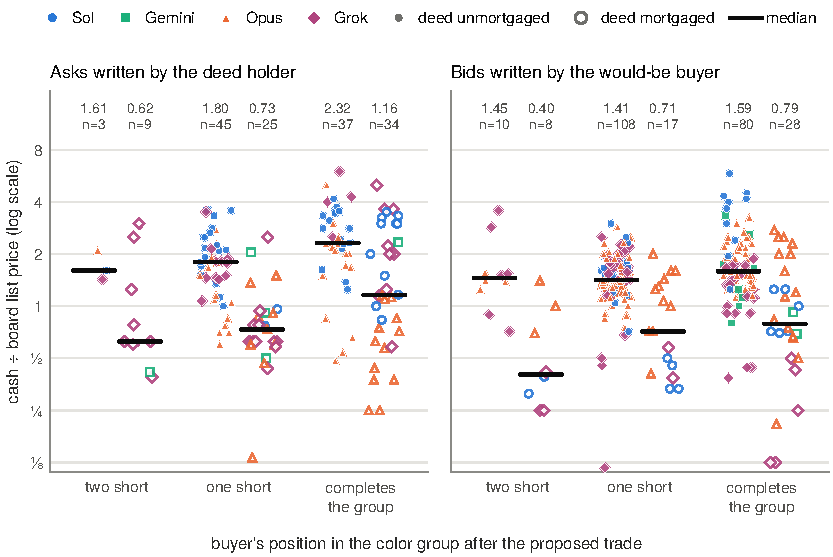
\includegraphics[width=\linewidth]{fig_prices.pdf}
\caption{Cash prices for a single color-group deed, as a multiple of board list price. Each point is one acceptance-legal offer, colored by the system that wrote it. Asks rise as the buyer nears a complete group. Bids rise little. Offers within a thread or game are dependent, and deed mix and game state differ across columns.}
\label{fig:prices}
\end{figure}

Asks rise as the buyer nears a complete group. For unmortgaged deeds the median ask is \fact{d.grad.ask.unmortgaged.2.median} times list when the buyer would still lack two deeds, \fact{d.grad.ask.unmortgaged.1.median} when it would lack one and \fact{d.grad.ask.unmortgaged.0.median} when the deed completes the group. Mortgaged deeds show the same order at lower levels. Bids move much less, with medians of \fact{d.grad.bid.unmortgaged.2.median}, \fact{d.grad.bid.unmortgaged.1.median} and \fact{d.grad.bid.unmortgaged.0.median} for unmortgaged deeds. For a completing, unmortgaged deed the median ask is therefore \fact{d.grad.ask.unmortgaged.0.median} times list and the median bid \fact{d.grad.bid.unmortgaged.0.median}.

The direction of the ask pattern is stable across coarse cuts. Asks to a completing buyer are higher in all \fact{barg.prices.cells-with-at-least-3-each.ask.higher} seller and mortgage-status cells with at least three asks on each side (Appendix~\ref{app:bargaining}), in all \fact{d.ask.stagecells.n} cells formed by thread position and mortgage status, and in \fact{d.ask.blocks.higher} of the 5 seed blocks for unmortgaged deeds. With any one block left out, the median unmortgaged ask stays between \fact{d.ask.lobo.comp.min} and \fact{d.ask.lobo.comp.max} for completing buyers and between \fact{d.ask.lobo.other.min} and \fact{d.ask.lobo.other.max} for others. Bids show no common direction. Sol bids \fact{d.price.bid.Sol.unmortgaged.completes} times list for a deed that completes its own group against \fact{d.price.bid.Sol.unmortgaged.other} otherwise, and Grok bids \fact{d.price.bid.Grok.unmortgaged.completes} against \fact{d.price.bid.Grok.unmortgaged.other}.

The tightest comparison is weaker. In \fact{d.pairs.n} cases one seller prices one deed, within one game, for both a completing and a non-completing buyer. The completing buyer is asked more in \fact{barg.prices.same-game-seller-deed-direction.higher} cases, less in \fact{barg.prices.same-game-seller-deed-direction.lower} and the same in \fact{barg.prices.same-game-seller-deed-direction.equal} (Table~\ref{tab:pairs}). Both of the lower cases are Opus selling Boardwalk as its cash ran down. We therefore report a consistent direction and do not estimate a premium. Counteroffers add a caution. A counter usually keeps the bundle and asks for more cash, and it does so about as often when no one would complete a group (\fact{barg.counters.neither-with-deed-request.same-noncash-bundle-more-cash-to-counterer} of \fact{barg.counters.neither-with-deed-request.counters} counters) as when the original author would (\fact{barg.counters.author-only.same-noncash-bundle-more-cash-to-counterer} of \fact{barg.counters.author-only.counters}). Repricing is how these agents bargain in general. What is specific to completing deeds is the level of the ask and the frequency of outright refusal.

\subsection{What the refusals say}

Two earlier model-assisted readings coded the stated reasons in all \fact{inh.reason.rows} outright rejections of offers that would complete the recipient's own group. Both found a stated consequence for the rival, such as its completion, building funds or survival, in \fact{inh.reason.D.both} (Cohen's $\kappa$ of \fact{inh.reason.D.kappa} between the readings). Both found a stated concern about the recipient's own cash, price or reserves in \fact{inh.reason.C.both} ($\kappa$ of \fact{inh.reason.C.kappa}). The rival code covers \fact{inh.reason.D.both.recipient-only} of the \fact{inh.reason.rows.recipient-only} refusals of offers completing only the recipient's group. By recipient it covers \fact{inh.reason.D.both.Gemini} of \fact{inh.reason.rows.Gemini} for Gemini, \fact{inh.reason.D.both.Grok} of \fact{inh.reason.rows.Grok} for Grok, \fact{inh.reason.D.both.Sol} of \fact{inh.reason.rows.Sol} for Sol and \fact{inh.reason.D.both.Opus} of \fact{inh.reason.rows.Opus} for Opus, whose eight records have no private note. Two games supply \fact{inh.reason.rows.top2games} of the \fact{inh.reason.rows} refusals. The readings came from two instances of one model family, one of them partly exposed to earlier counts, and no human labeled the rows. They establish what the messages and notes say and not why the agents refused. The two incidents below show the content behind the codes.

\IncidentTitle{g2}{A blocker kept while its holder is liquid and has nothing to build (G2)}

At G2 turn 44 Sol holds Marvin Gardens, \$137 and no complete group. Opus holds the other two yellows. Grok owns no yellow and bids \$200.
\TranscriptQuote{g2-d118-liquidity-pitch}
Sol asks \$450 and rejects Grok's \$250. One turn later Opus bids \$325 for the same deed, which would complete its yellows. Sol asks \$650.
\TranscriptQuote{g2-d124-price}
\TranscriptQuote{g2-d124-note}
Sol comes down to \$600 and Opus stops at \$450. Sol's note on its final rejection gives the reason for keeping the deed.
\TranscriptQuote{g2-d128-note}
Twenty-four turns later the positions have reversed. Sol has \$435 and Opus \$17. Sol offers two railroads for Opus's two mortgaged yellows, and Opus replies.
\TranscriptQuote{g2-d197-reverse}
\IncidentOutcome{Sol pays the extra \$100 and completes yellow. Opus is eliminated three turns later owing Gemini \$1,300. Sol builds two houses, sells them four turns after the trade to pay rent, and is eliminated at turn 85. Both estates pass to Gemini, which wins.}
\IncidentReading{Sol prices one deed at \$450 for a buyer with no yellows and \$650 for the buyer it would complete, and its note counts that buyer's remaining building cash. The \$520 figure is right and the house count is wrong, since \$520 buys three yellow houses, and house prices are absent from the prompt at this decision. Both bidders pitch liquidity to a seller holding \$137. Sol declines because it can mortgage other deeds and has no group on which to spend the proceeds. Once Opus is down to \$17, the group changes hands in the other direction.}
\IncidentSource{G2 d118--d128 and d196--d198. Sol and Grok respond under the standard condition. Opus's d197 message is an action-only response. Quoted public messages appear in the named counterparty's next prompt.}

\IncidentTitle{g15}{Refusing one's own complete group three times (G15)}

At G15 turn 63 Sol has \$730 and Grok \$333. One turn earlier Opus had addressed the table.
\TranscriptQuote{g15-d166-appeal}
Sol offers Grok its two greens for Ventnor and \$100. The trade would complete green for Grok and yellow for Sol. Grok refuses, and its note compares what each side could then build.
\TranscriptQuote{g15-d169-refusal-note}
Sol drops its cash request and adds Kentucky. When Grok refuses again, Sol adds \$250 of its own.
\TranscriptQuote{g15-d174-sweetener}
\TranscriptQuote{g15-d175-final-refusal}
Sol's closing note says when it will try again.
\TranscriptQuote{g15-d176-wait-note}
\IncidentOutcome{No trade settles. In the same turn Gemini refuses to sell Sol the deed that would complete light blue. Eighteen turns later Grok is the first player eliminated, and its yellow and green blockers pass to Gemini, which wins. Sol never completes either group.}
\IncidentReading{Grok turns down its own complete group three times because of what the same trade would let Sol build, and Sol reshapes its offer around that objection. Grok's cash arithmetic matches the ledger, though its \$600 is the price of a full first layer on green and one green house costs \$200. The refusals kept two blockers from Sol until Grok's bankruptcy handed them to a third player. Sol's last note states the timing rule that the next section finds in the population.}
\IncidentSource{G15 d166--d176. Opus's appeal is an action-only response and appears in Grok's d169 prompt. All other quoted responses are standard first attempts.}
